\section{Лекція 1: Знайомство з Python}
 
\begin{frame}
\frametitle{Викладач}
\begin{wrapfigure}{r}{0.35\textwidth}
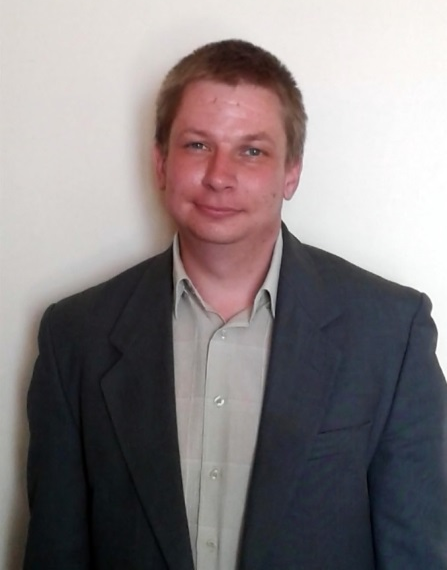
\includegraphics[width=0.25\textwidth]{pictures/myphoto}
\caption{Легенький М.М.}
\label{myphoto}
\end{wrapfigure}
\textbf{Легенький Максим Миколайович}

доцент кафедри теоретичної радіофізики

\textit{факультету радіофізики, біомедичної електроніки та комп’ютерних систем}

aуд. 5-5

тел. (057) 707-52-57

e-mail: \href{mailto:mlegenkiy@karazin.ua}{mlegenkiy@karazin.ua}

Telegram: \href{https://t.me/mlegenkiy}{@mlegenkiy}
\end{frame}

\begin{frame}
\frametitle{Python}
% 	\frametitle{\insertsection} 
% 	\framesubtitle{\insertsubsection}
\begin{wrapfigure}{r}{0.35\textwidth}
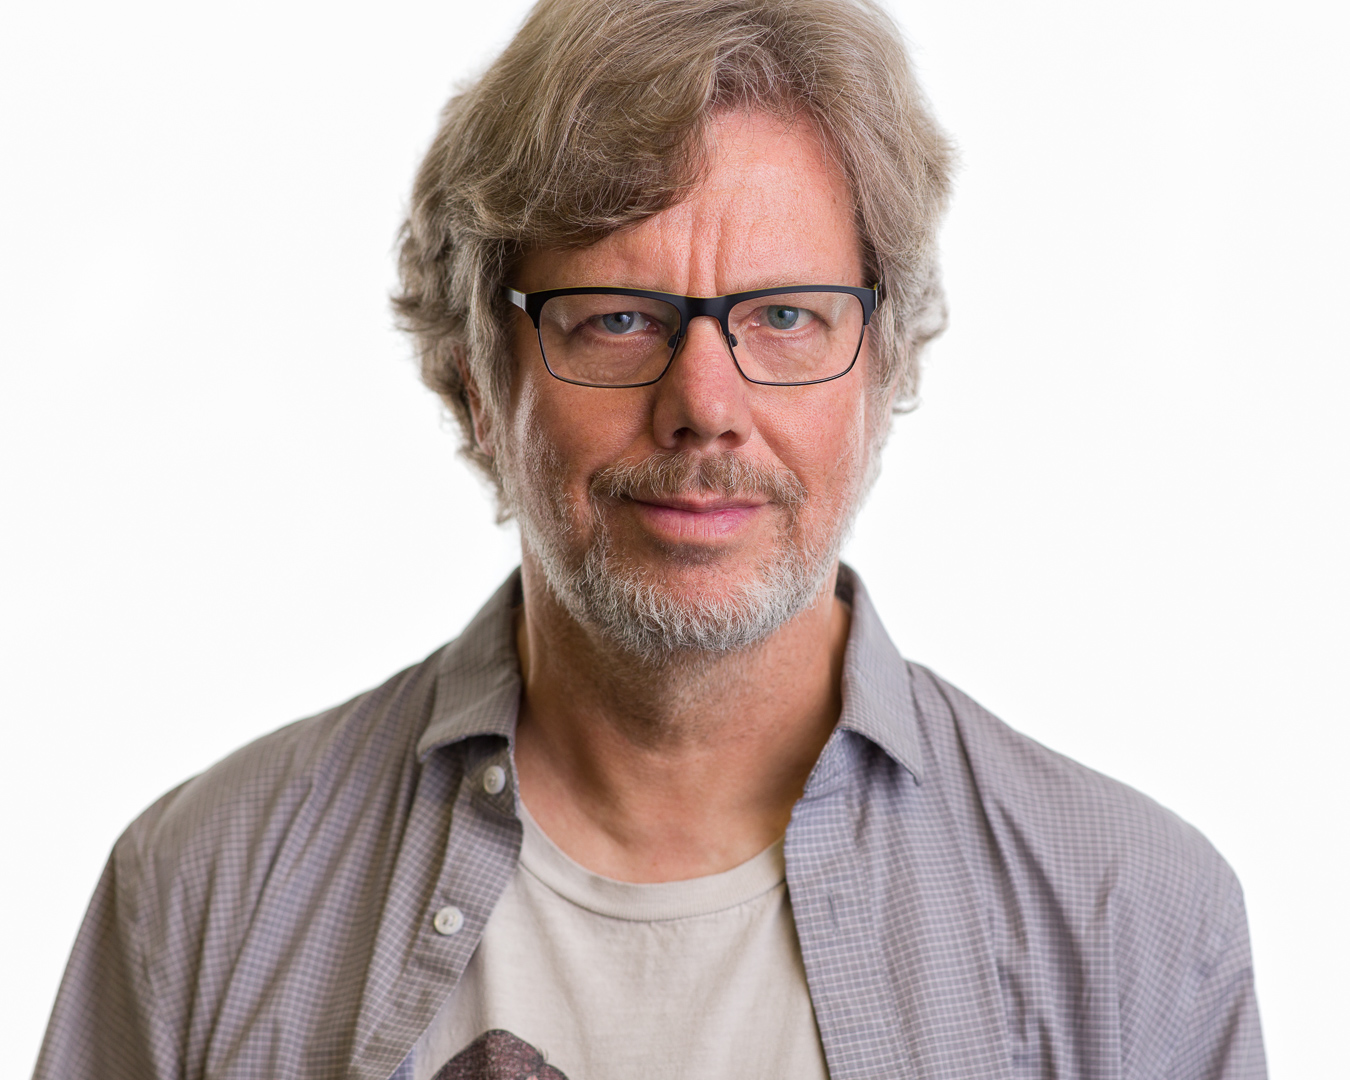
\includegraphics[width=0.25\textwidth]{pictures/guido}
\caption{Гвідо ван Россум}
\label{gvido}
\end{wrapfigure}
Python (Пайтон) — інтерпретована об'єктно-орієнтована мова програмування високого рівня зі строгою динамічною типізацією.  Назву запозичено із назви британського шоу Монті Пайтон. Розроблена в 1990 році Гвідо ван Россумом. 
\end{frame}

\begin{frame}
\frametitle{Версії Python}
%\begin{wrapfigure}{r}{0.35\textwidth}
\begin{figure}
  \begin{center}
    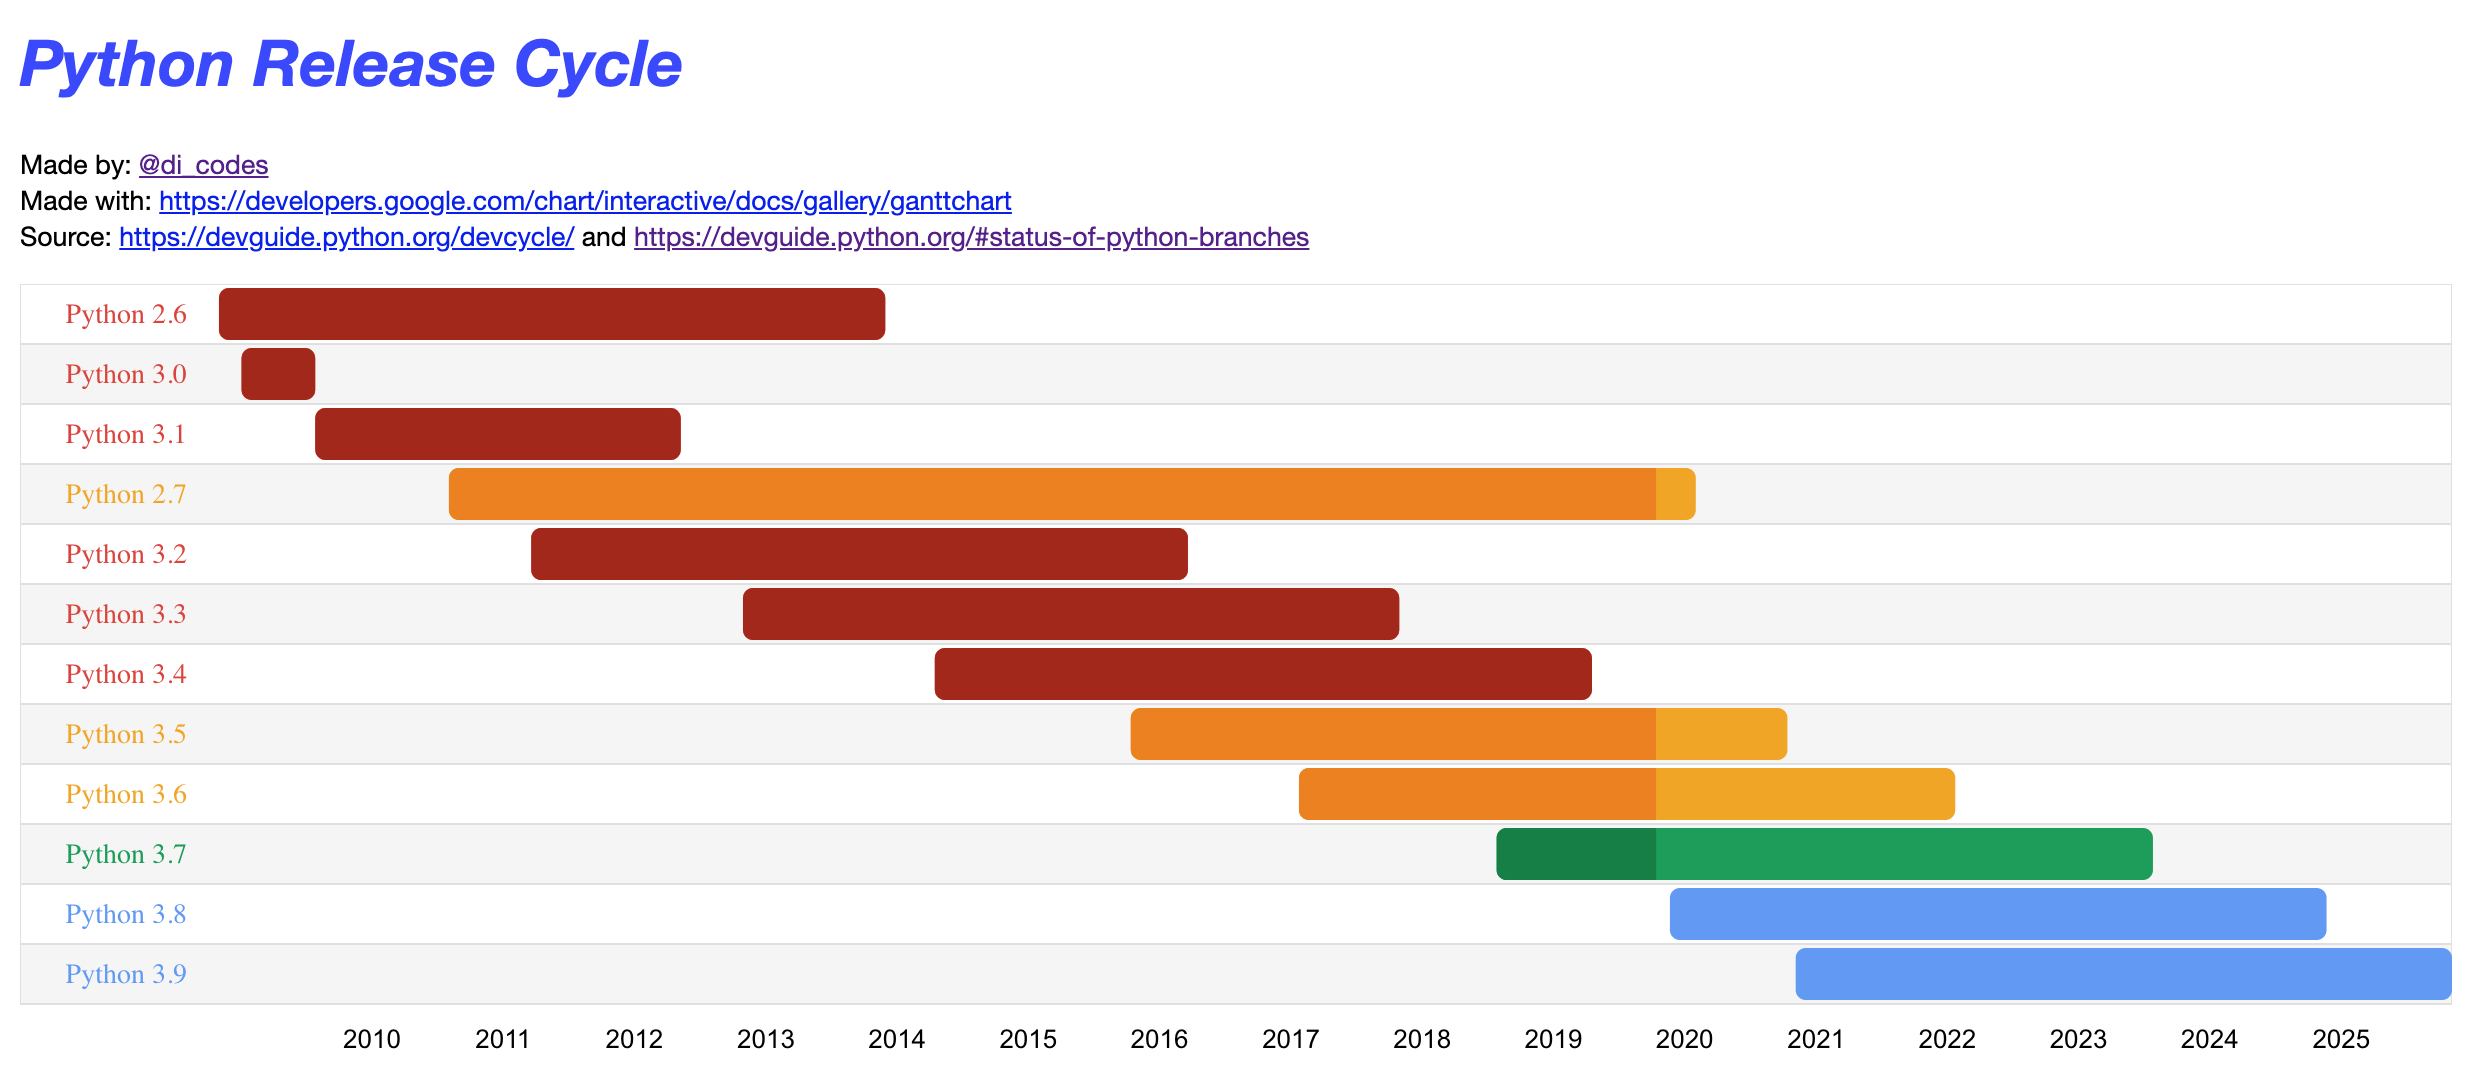
\includegraphics[width=\textwidth,height=0.5\textheight]{pictures/python_versions}
  \caption{Версії Python та період їх підтримки}
\label{versions}
  \end{center}
\end{figure}

%\end{wrapfigure}

\end{frame}

\begin{frame}
\frametitle{Переваги та недоліки Python}
Переваги:
\begin{itemize}
  \item зручність та простота програмування;
  \item переносимість програм;
  \item велика кількість модулів;
  \item поширеність та популярність.
\end{itemize}
Недоліки:
\begin{itemize}
  \item порівняно низька швидкість виконання програм;
  \item неможливість модифікації вбудованих класів.
\end{itemize}
\end{frame}

\begin{frame}
\frametitle{Сайт Python}
\begin{figure}
\begin{center}
 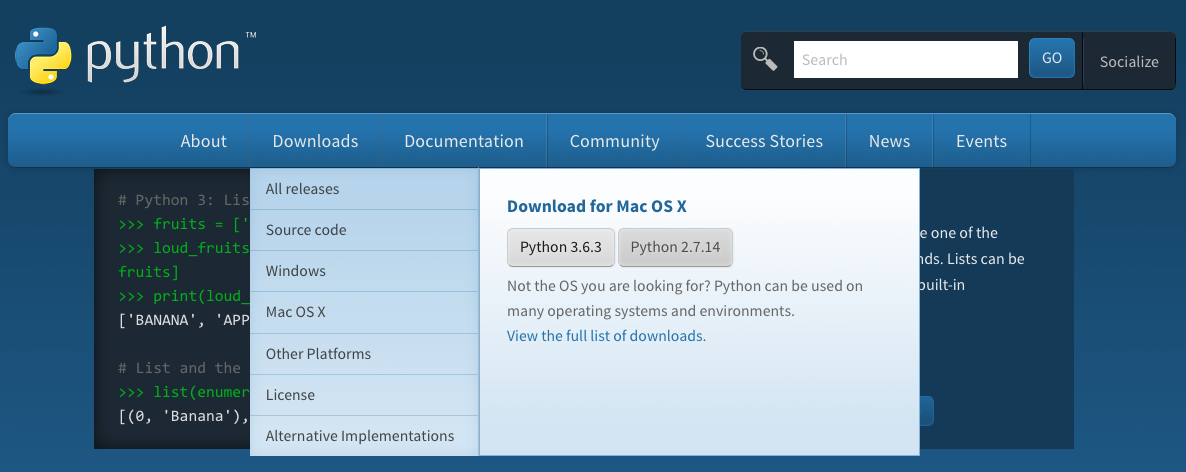
\includegraphics[width=0.95\textwidth]{pictures/python_site.png}
\caption{Сайт: \href{https://python.org/}{python.org}}
\label{python_site} 
\end{center}
\end{figure}

\end{frame}

\begin{frame}
\frametitle{Встановлення Python}
\begin{figure}
\begin{center}
 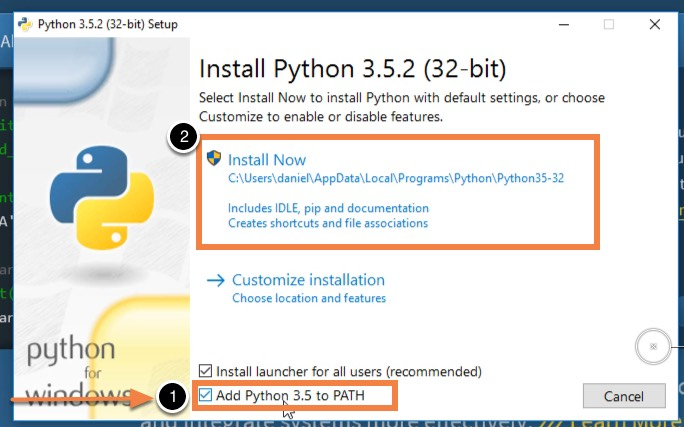
\includegraphics[width=0.7\textwidth]{pictures/python_install.jpg}
\caption{Встановлення Python}
\label{python_install} 
\end{center}
\end{figure}
\end{frame}

\begin{frame}
\frametitle{Виконання коду Python}
\begin{itemize}
  \item інтерактивний;
  \item файловий.
\end{itemize}
\textbf{PEP 8} – Style Guide for Python Code
\end{frame}

\begin{frame}
\frametitle{PyCharm}

\begin{wrapfigure}{r}{0.4\textwidth}

\includegraphics[width=0.25\textwidth]{pictures/pycharm_logo.png}
\caption{Логотип PyCharm}
\label{pycharm_logo}
\end{wrapfigure}


\textbf{PyCharm} — інтегроване середовище розробки для мови програмування Python. \href{https://www.jetbrains.com/pycharm/download/}{Сайт} для завантаження PyCharm.
\end{frame}

